%TODO Change hash information to include speech-marks
\newpage
\section{Definition of Mass Transfer}

\subsection*{Resources}
\begin{itemize}
    \item Chapter 14, introduction
\end{itemize}

\subsection*{Challenge}
Add the points of the following conditions which constitute diffusive mass-transfer

1 point: Evaporation of water vapour into the air

2 points: Water being pumped through a pipe

4 points: Dissolving of sugar into tea

8 points: Aeration of waste-water

16 points: Motion of air around a room due to the presence of a fan

\subsection*{Solution}
(Enter as an integer)

\hash{a}{b786dd}




\newpage
\section{Diffusion in the long time limit}

\subsection*{Resources}
\begin{itemize}
    \item Book: 14.1.1 to 14.1.2
    \item Video: \url{https://www.youtube.com/watch?v=-FLv0uxLrDI}
\end{itemize}

\subsection*{Challenge}
Consider a box of volume \SI{1}{\cubic\meter}. The box contains 1 mole of gas. At time $t=0$, all the gas molecules in the left 1/4 of the box are labeled $A$. As time goes to $t=\infty$, what will the density of the molecules labeled $A$ be in the right half of the box? Note that there is only 1 species of gas in the box.

\subsection*{Solution}
Units: Moles / $m^3$

(enter to two decimal places)

\hash{b}{13c60a}




\newpage
\section{Definitions of quantities I}

\subsection*{Resources}
\begin{itemize}
    \item Book: 14.1.1 to 14.1.2
    \item Video: \url{https://www.youtube.com/watch?v=-FLv0uxLrDI}
\end{itemize}

\subsection*{Challenge}
Assuming air is made up exclusively of oxygen and nitrogen with their partial pressures in the ratio 0.21:0.79, what are their mass-fractions?

\subsection*{Solutions}
Oxygen: 0.233 \\
Nitrogen: 0.767




\newpage
\section{Definitions of quantities II}

\subsection*{Resources}
\begin{itemize}
    \item Book: 14.1.1 to 14.1.2
    \item Video: \url{https://www.youtube.com/watch?v=-FLv0uxLrDI}
\end{itemize}

\subsection*{Challenge}
Japan imports substantial amounts of LNG which is a mixture of the following gases:

\begin{tabular}[c]{|c|c|}
    \hline
    \textbf{Liquid} & \textbf{Mol \%}\\
    \hline
    Methane         & 93.5  \\
    Ethane          & 4.6   \\
    Propane         & 1.2   \\
    Carbon dioxide  & 0.7   \\
    \hline
\end{tabular}

The masses of Methane, Ethane, Propane and Carbon Dioxide are 16, 30, 44 and 44 g/mol respectively.

Assuming ideal gases, calculate the following:

1. The mole-fraction of ethane

2. The mass-fraction of ethane

3. The average molecular mass of the mixture

4. The mass-density of the gas when heated to \SI{207}{\kelvin} under a total pressure of \SI{1.4e5}{\pascal}

5. The partial pressure of the methane when the total pressure is \SI{1.4e5}{\pascal}

\subsection*{Solutions}

1. (enter as a decimal to 3 decimal places) \hash{c}{117398}

2. (enter as a decimal to 3 decimal places) \hash{d}{6801da}

3. (enter as a decimal to 3 decimal places in units of g/mol) \hash{e}{e3a65e}

4. \SI{1397}{\kg\per\cubic\meter}

5. (enter as an integer in units of kPa) \hash{f}{f54c28}




\newpage
\section{Mass diffusivity}

\subsection*{Resources}
\begin{itemize}
    \item Book: 14.1.3 - 14.1.4, Table A-8
\end{itemize}

\subsection*{Challenge}
Estimate the mass diffusivity of the following gases in air at 350 K and 1 atm pressure:

1. Ammonia\\
2. Hydrogen

\subsection*{Solutions}
1. \SI{0.36e-4}{\square\meter\per\second}\\
2. \SI{0.52e-4}{\square\meter\per\second}




\newpage
\section{Cases of diffusion}

\subsection*{Resources}
\begin{itemize}
    \item Book: 14.1.3 - 14.1.4
\end{itemize}

\subsection*{Challenge}
Considering air in a closed, cylindrical container with its axis vertical and with opposite ends maintained at different temperatures. Assume the total pressure of the air is uniform throughout the container.

Consider each of the following conditions:

1. The bottom surface is colder than the top surface\\
2. The top surface is colder than the bottom surface

For each condition, write a few sentences explaining a) if there is any motion of the air and b) if mass transfer occurs.

\subsection*{Solutions}
Please compare your answer with your partner.




\newpage
\section{Diffusion coefficient equivalency}

\subsection*{Resources}
\begin{itemize}
    \item Video: \url{https://www.youtube.com/watch?v=NTlR18NyqAE}
\end{itemize}

\subsection*{Challenge}
Prove that in a binary mixture, the diffusion coefficient of gas ``A'' in ``B'' is the same as the diffusion coefficient of gas ``B'' in ``A'' (ie, $D_{AB} = D_{BA}$).




\newpage
\section{Saturated water vapour pressure}

\subsection*{Resources}
\begin{itemize}
    \item \url{http://www.chemguide.co.uk/physical/phaseeqia/vapourpress.html}
\end{itemize}

\subsection*{Challenge}
Write a few sentences briefly explaining what is meant by ``Saturated Vapour Pressure''.

%2. As you increase in altitude above the earth, does this increase, decrease or stay the same?

\subsection*{Solution}
Compare your answer with your partner




\newpage
\section{Evaporation through a pore}

\subsection*{Resources}
\begin{itemize}
    \item Book 14.2 (be sure to follow the derivation of column evaporation)
\end{itemize}

\subsection*{Challenge}
In your challenge log, work through example 14.2 (you do not need to include the ``comments'' part in your challenge log).



% NT: Challenge about partial pressure and molar density conversion (LD2)
% NT: Challenge about humidity and partial pressure
% NT: Calculation challenge about V_g in table A-6


\newpage
\section{Evaporation pan}

\subsection*{Resources}
\begin{itemize}
    \item Book 14.2, Tables A-6 and A-8
    \item Challenges in Appendix A
\end{itemize}

\subsection*{Challenge}
Evaporation pans like the one shown are used to measure the rate of evaporation of water in a local area.

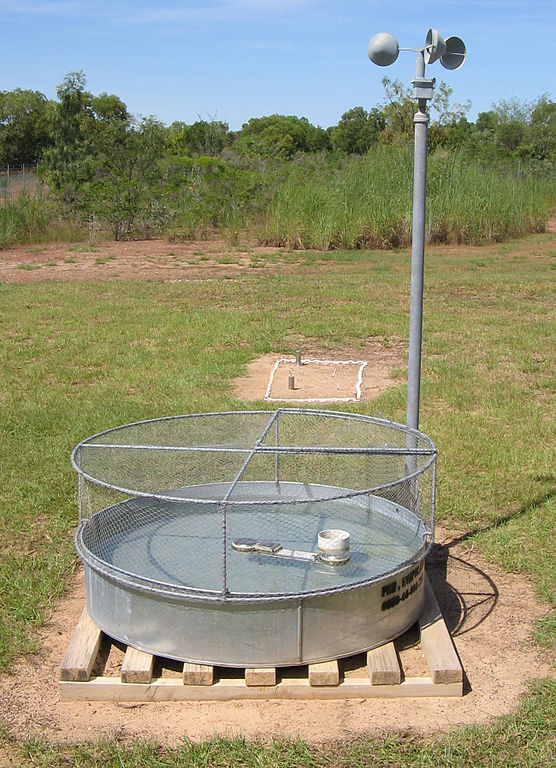
\includegraphics{evappan}
\emph{(image: \href{https://commons.wikimedia.org/wiki/File:Evaporation_Pan.jpg}{Bidgee, Wikipedia)}}

An evaporation pan is placed in a location with an ambient air temperature of \SI{300}{\kelvin} and relative humidity of 25\%. The pan contains water at the same temperature as the surrounding air. It has a diameter of \SI{20}{\cm} and height of \SI{160}{\mm}, and it starts half-full of water.

1. Assuming only diffusive mass transport, what is the initial evaporation rate?

2. Including the effects of advection, what is the initial evaporation rate?

%3. Determine how long it takes for all the water to evaporate.

\subsection*{Solution}
1. \SI{1.087e-8}{\kilo\mol\per\second}\\
2. \SI{1.107e-8}{\kilo\mol\per\second}





\newpage
\section{Stationary Medium}

\subsection*{Resources}
\begin{itemize}
    \item Video: \url{https://www.youtube.com/watch?v=F0deXOH_YEM}
\end{itemize}

\subsection*{Challenge}
\begin{enumerate}
    \item Briefly explain what is meant by a stationary medium.
    \item Considering a stationary medium of 3 species ``A'', ``B'' and ``C'', if the flux of species ``A'' is \SI{2}{\kmol\per\square\meter\per\second} and ``B'' is \SI{-8}{\kmol\per\square\meter\per\second}, what is the flux of species ``C''?
    \item Considering a binary system of atoms ``A'' and ``B'' with concentration \SI{5}{\kmol\per\cubic\meter} and \SI{10}{\kmol\per\cubic\meter} respectively, if the molar velocity of species ``A'' is \SI{2}{\meter\per\second}, what is the molar velocity of species ``B''?
\end{enumerate}



\subsection*{Solutions}
1. Please compare your answer with your partner

2. (enter to two decimal places in units of \si{\kmol\per\square\meter\per\second}) \hash{g}{2c32d8}

3. (enter to two decimal places in units of \si{\meter\per\second}) \hash{h}{3ccbb4}




\newpage
\section{Stationary Medium Approximation}

\subsection*{Resources}
\begin{itemize}
    \item Book 14.3
\end{itemize}

\subsection*{Challenge}
In a few sentences, describe what is meant by \emph{the stationary medium approximation}. Give at least one real-world example each of case where the stationary medium approximation would and would-not be appropriate.

\subsection*{Solution}
Compare your answer with your partner




\newpage
\section{Steady-state definition}

\subsection*{Resources}
\begin{itemize}
    \item Web: \url{http://www.virginia.edu/bohr/mse209/chapter5.htm}
\end{itemize}

\subsection*{Challenge}
The example in section 14.4.3 talks of steady state conditions.

1. Write a sentence or two explaining what is meant by steady-state conditions in this context.

2. What is $\delta J(x) / \delta t$ at any given position $x$ under a steady-state condition?

\subsection*{Solutions}
1. Please compare your answer with your partner

2.\\
X = Your solution\\
Form: Decimal, to 1 decimal place\\
Place the indicated letter in front of the number\\
Example: aX where $X=42.5$ is entered as \href{http://www.wolframalpha.com/input/?i=md5+hash+of+\%22a42.5\%22}{a42.5}

hash of aX = 9497cd




\newpage
\section{Steady-state diffusion planer example I}

\subsection*{Resources}
\begin{itemize}
    \item Book: 14.4.1 to 14.4.3
    \item Video: \url{https://youtu.be/4KACai1gYzc}
\end{itemize}

\subsection*{Challenge}
Work through the calculation from equations 14.51 to 14.54, showing your reasoning along the way. Don't worry about the concept of diffusion resistance for now.




\newpage
\section{Steady-state diffusion planer example II}

\subsection*{Resources}
\begin{itemize}
    \item Book: 14.4.1 to 14.4.3
    \item Video: \url{https://youtu.be/4KACai1gYzc}
\end{itemize}

\subsection*{Challenge}
Work through example 14.3 in section 14.4.3.




\newpage
\section{Steady-state diffusion through flat surface}

\subsection*{Resources}
\begin{itemize}
    \item Book: 14.4.1 to 14.4.3
\end{itemize}

\subsection*{Challenge}
A thin plastic membrane is used to maintain separation between helium and an outer chamber. Under steady-state conditions, the concentration of helium is \SI{0.02}{\kmol\per\cubic\meter} and \SI{0.005}{\kmol\per\cubic\meter} at the inner and outer boundaries respectively. If the membrane is \SI{1}{\mm} thick and the binary diffusion coefficient of helium in the plastic membrane is \SI{e-9}{\square\meter\per\second}, what is the diffusive flux through the membrane in terms of \si{\kmol\per\second\per\square\meter} and \si{\kg\per\second\per\square\meter}?

\subsection*{Solution}
\SI{1.5e-8}{\kmol\per\second\per\square\meter}\\
\SI{6.0e-8}{\kg\per\second\per\square\meter}




\newpage
\section{Steady-state diffusion in pipe walls}

\subsection*{Resources}
\begin{itemize}
    \item Book: 14.4.1 to 14.4.3
\end{itemize}

\subsection*{Challenge}
A pipe with inner-radius \SI{10}{\cm} and outer-radius \SI{13}{\cm} is carrying hydrogen. The concentration of hydrogen inside the pipe is \SI{0.07}{\kmol\per\cubic\meter} and outside the pipe is \SI{0.04}{\kmol\per\cubic\meter}. If the hydrogen has a diffusion coefficient of \SI{e-8}{\square\meter\per\second} in the walls of the pipe, at what rate is hydrogen lost from the pipe, per metre length of pipe?

\subsection*{Solution}
\SI{7.18e-9}{\kmol\per\second}




\newpage
\section{Raoult's law}

\subsection*{Resources}
\begin{itemize}
    \item Book: 14.5.1
\end{itemize}

\subsection*{Challenge}
Considering a puddle of water exposed to the atmosphere at \SI{17}{\celsius}, calculate:

1. The molar fraction of water vapour on the air-side of the water-air interface.\\
2. The mass fraction of water vapour on the air-side of the water-air interface.\\
3. The molar fraction of water vapour on the water-side of the water-air interface.\\
4. The mass fraction of water vapour on the water-side of the water-air interface.

\subsection*{Solution}
1. \num{0.019}

2. \num{0.012}

3.\\
X = Your solution\\
Form: Decimal, to 3 decimal places\\
Place the indicated letter in front of the number\\
Example: aX where $X=42.544$ is entered as \href{http://www.wolframalpha.com/input/?i=md5+hash+of+\%22a42.544\%22}{a42.544}

hash of bX = 4b5ab9

4.\\
X = Your solution\\
Form: Decimal, to 3 decimal places\\
Place the indicated letter in front of the number\\
Example: aX where $X=42.544$ is entered as \href{http://www.wolframalpha.com/input/?i=md5+hash+of+\%22a42.544\%22}{a42.544}

hash of cX = 737b49

